%%%%%%%%%%%%%%%%%%%% author.tex %%%%%%%%%%%%%%%%%%%%%%%%%%%%%%%%%%%
%
% sample root file for your "contribution" to a contributed volume
%
% Use this file as a template for your own input.
%
%%%%%%%%%%%%%%%% Springer %%%%%%%%%%%%%%%%%%%%%%%%%%%%%%%%%%


% RECOMMENDED %%%%%%%%%%%%%%%%%%%%%%%%%%%%%%%%%%%%%%%%%%%%%%%%%%%
\documentclass[graybox]{svmult}

% choose options for [] as required from the list
% in the Reference Guide

\usepackage{mathptmx}       % selects Times Roman as basic font
\usepackage{helvet}         % selects Helvetica as sans-serif font
\usepackage{courier}        % selects Courier as typewriter font
\usepackage{type1cm}        % activate if the above 3 fonts are
                            % not available on your system
%
\usepackage{makeidx}         % allows index generation
\usepackage{url}             % links
\usepackage{graphicx}        % standard LaTeX graphics tool
                             % when including figure files
\usepackage{multicol}        % used for the two-column index
\usepackage[bottom]{footmisc}% places footnotes at page bottom

\usepackage{algorithm}
\usepackage[noend]{algpseudocode}

% see the list of further useful packages
% in the Reference Guide

\makeindex             % used for the subject index
                       % please use the style svind.ist with
                       % your makeindex program

%%%%%%%%%%%%%%%%%%%%%%%%%%%%%%%%%%%%%%%%%%%%%%%%%%%%%%%%%%%%%%%%%%%%%%%%%%%%%%%%%%%%%%%%%

\begin{document}

\title*{Accelerated Load Balancing of Unstructured Meshes}
% Use \titlerunning{Short Title} for an abbreviated version of
% your contribution title if the original one is too long
\author{
Gerrett Diamond,
Lucas Davis,
Cameron W. Smith,
and Mark S. Shephard
}
\institute{
  Gerrett Diamond \email{diamog@rpi.edu}
  \and Lucas Davis \email{davisl3@rpi.edu}
  \and Cameron W. Smith \email{smithc11@rpi.edu}
  \and Mark S. Shephard \email{shephard@rpi.edu}
  \at Rensselaer Polytechnic Institute, Troy, NY 
}
\authorrunning{G.Diamond et al.}

\maketitle

\abstract{
  gpus are in lots of big systems, we need to use them for load balancing
}

\section{Introduction} \label{sec:intro}

\begin{itemize}
  \item briefly motivate dynamic load balancing
  \item quantify how GPUs are providing the majority of computing performance (\# of systems with GPUs in top 10 systems of top500, graph500, HPCG)
  \item end with a sentence that says what engpar does (diffusion) and how we are
extending it to run on GPUs
\end{itemize}

Unstructured mesh applications running on current and next generation machines require the
computational work related to mesh entities to be evenly distruibuted across processes in
order to achieve maximal performance. While common partitioning techniques such as multilevel
[REFERENCES] or geometric [REFERENCES] methods are good for creating an initial distribution
of load, evolving simulations where the mesh and computational load changes during the
simulation require dynamic load balancing techniques that are quick to improve the partition
as the work load changes. Diffusive load balancing methods allow quick partition refinement
for the relatively small changes to imbalance that are seen in adaptive mesh simulations.

\section{EnGPar Dynamic Load Balancing} \label{sec:engpar}

\begin{itemize}
  \item multi-graph, high-level diffusion algorithm (targeting, selection, migration)
  \item indicate that we will accelerate selection via BFS for distance computation and coloring for cavity selection
\end{itemize}

\subsection{N-graph}

EnGPar is a partition improvement tool that utilizes a specialized multi-hypergraph,
called the N-graph, to describe the portions of the mesh that require load balancing.
The N-graph consists of vertices which represent the primary dimension entities of the
mesh. The vertices are connected by hyperedges created from the secondary dimensions of
the mesh that require load balancing. Figure \ref{fig:ngraph} shows the conversion from
mesh (a) to hypergraph (b) where mesh faces are used to create the graph vertices and
mesh vertices are represented by hyperedges. A second edge type is used to represent mesh edges in (c). 

\begin{figure}[!ht]
  \centering
  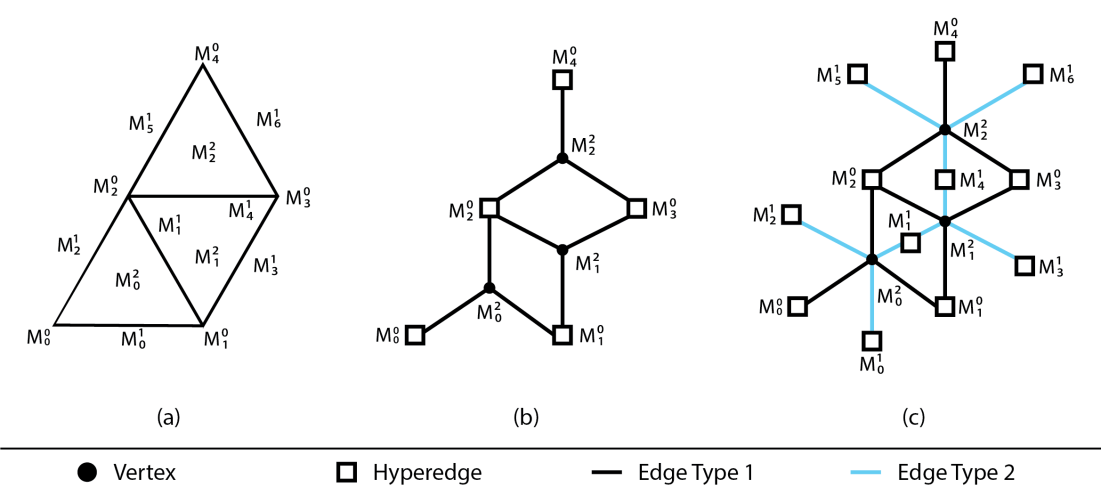
\includegraphics[width=3.5in]{images/exampleMesh2Graph.png}
  \caption{A triangular mesh (a) converted to the N-graph with mesh faces represented by graph vertices and mesh vertices as hyperedges (b) and mesh edges as a second hyperedge type (c).}
  \label{fig:edgecounts}
\end{figure}


\subsection{Diffusive Load Balancing}

EnGPar's diffusive algorithm is an iterative local refinement strategy where in each
iteration the target criteria is improved until the imbalance is under a given
tolerance or the imbalance cannot be improved further. Each iteration consists of three
steps: targeting, selection, and migration.
Algorithm~\ref{alg:engpar} lists the pseudo code.
The targeting phase consists of gathering
metrics on the part and its neighbors in order to determine which neighboring parts to
send weight to and how much weight to send. The selection step is where graph vertices
on the boundary are chosen to be sent to neighboring parts in order to satisfy the
weights determined by the targeting phase. Finally, the migration phase sends the graph
entities that were selected to the destination parts and the graph is reconstructed.

\begin{algorithm}[H]
  \caption{Diffusive Load Balancing Framework}
  \label{alg:engpar}
  \small
  \begin{algorithmic}[1]
    \Procedure{Balance}{$ngraph$,$entity\_types$}
    \ForAll{$t \in entity\_types$}
    \While{imbalance of $t >$ tolerance}
    \Call{RunStep}{$ngraph$,$t$}
    \If{Balancing Stagnates}
    \State break
    \EndIf
    \EndWhile
    \EndFor
    \EndProcedure

    \Procedure{RunStep}{$ngraph$,$t$}
    \State $sides = makeSides(ngraph)$
    \State $weights = makeWeights(ngraph,sides,t)$
    \State $targets = makeTargets(ngraph,sides,weights)$
    \State $queue = makeQueue(ngraph)$
    \State $plan = select(ngraph,targets,queue)$
    \State $ngraph.migrate(plan)$
    \EndProcedure
  \end{algorithmic}
\end{algorithm}

In this work, we target accelerating two sections of the selection phase. The first is
the distance computation where hyperedges on the boundary are ordered based on their
distance from the center of the part from furthest to closest.
{\color{red}Should give more details as to why this is important.}
The second is the selection of which cavities, defined by a hyperedge and the
vertices that are connected by it, on the part boundary to send to neighboring parts.

{\color{red} We could add one of the cavity images from the presentations?}

%A cavity is formed by a hyperedge and the vertices pinned to it.

\section{Accelerating Distance Computation} \label{sec:dist}

provide results - serial vs kokkos w/cuda -
\url{https://bitbucket.org/c_smith/engpar_siampp18/src/master/}

\section{Accelerating Cavity Selection} \label{sec:select}

Accelerating the selection of cavities requires simulateously evaluating many
cavities simultaneously.
The current single threaded selection procedure evaluates cavities in order of
their descending distance from the topological center.
Since the ordered selection exposes no concurrency an alternative application of
the topological distance is needed.
One approach is to bin the cavities by distance.
For large parts, or parts with high surface area, this will expose a modest
amount of concurrency.
A second approach applies the topological distance sorting after a fully
parallel cavity evaluation has executed.
Given that this approach provides maximum concurrency during cavity evaluation,
and can use a data-parallel sorting operation, it is the procedure used in this
work.

Critical to concurrent cavity evaluation is avoiding race conditions when
writing and reading the integer associated with each graph vertex indicating
which process they will be migrated to.
Hyperedge coloring ensures that any two hyperedges that share a common vertex
will be assigned a different color.
Hyperedges with the same color can be evaluated concurrently without
race conditions.

{\color{red}A figure showing hyperedge cavity selection and conflicts would be
helpful}

Kokkos-kernels data-parallel graph coloring procedure REFERENCE is used to
color the hyperedges of the EnGPar hypergraph.

Transforming the hypergraph to the symmetric adjacency matrix required as input
to the coloring procedure requires creating the dual of the hypergraph.
The dual graph represents the second adjacencies of
hyperedge-to-vertex-to-hyperedge (herein referred to as `EVE') by creating one
vertex for each hyperedge, and an edge between two hyperedges if they share at
least one common vertex.
Kokkos-kernel's graph coloring algorithm is then called to color this dual graph
which returns a coloring of the original graph's hyperedges.

\subsubsection{Parallel EVE Construction}

The construction of the second adjacency compressed matrix starts by making an
matrix that stores hyperedge-to-hyperedge adjacencies.
Because the information being read and written should not overlap or change due
to race conditions multiple levels or parallelism can be leveraged to improve
performance.
Then the matrix is converted to compressed row storage form using two single
dimension arrays, \verb|deg| and \verb|edgelist|.
Because \verb|deg| stores cumulative number of entries by row, a parallel
reduction is utilized to find the total number of entries in a row then a
parallel prefix sum  modifies the \verb|deg| array to store the total number of
entries up to row \verb|i| exclusively.
\verb|edgelist| stores the column index of the non-zero matrix entries which are
the hyperedge labels in this construction.
\verb|edgelist| stores the column index of each entry in row-major order.

\begin{verbatim}
edge_vertex_edge_adjacencies(G):
  parallel for each vertex
    for i in hyperedges(v)
      for j!=i in hyperedges(v)
        numAdj += 1 
  // value set to void works as True/False indicator
  Kokkos::UnorderedMap<Kokkos::pair<uint,uint>,void> m (numAdj)
  parallel for each vertex
    for i in hyperedges(v)
      for j!=i in hyperedges(v)
        Kokkos::pair<uint,uint> p( i , j )
        m.insert(p)       
  N = |E|
  deg = [N+1]
  deg(0) = 0
  parallel for each key in m
    Kokkos::pair<uint,uint> p = m.get(i).key 
    deg(p.first+1)++; //atomic add    
  parallel prefix sum 
    deg(i) = sum(deg(j=0,i))  
  edgeList = [deg(N)]
  adjCount = [N]
  parallel for each key in m
    Kokkos::pair<uint,uint> p = m.get(i).key
    e = degS(p.first)
    idx = adjCount(p.first)++
    edgeListS(e+idx) = p.second
\end{verbatim}


\subsubsection{Coloring Call}
{\small
\begin{verbatim}
agi::lid_t EnGPar_KokkosColoring(ColoringInput* in, agi::lid_t** colors) {
  agi::PNgraph* pg = in->g->publicize();
  // Retrieve relavent information from graph  
  agi::lid_t* adj_offsets = nullptr;
  agi::lid_t* adj_lists = nullptr;
  agi::lid_t numEnts = 0;
  if (in->primaryType == VTX_TYPE) {
    // Vertex colorings
    double t0 = PCU_Time();
    in->g->create_vev_adjacency(in->edgeType);
    printf ("eve partition time: %f\n", PCU_Time()-t0);
    numEnts = in->g->numLocalVtxs();
    adj_offsets = pg->vev_offsets[in->edgeType];
    adj_lists = pg->vev_lists[in->edgeType];
  } else {
    // Edge coloring
    double t0 = PCU_Time();
    //in->g->create_eve_adjacency(in->edgeType);
    parallel_create_eve(in->g, in->edgeType);
    printf ("eve partition time: %f\n", PCU_Time()-t0);
    numEnts = pg->num_local_edges[in->edgeType];
    adj_offsets = pg->eve_offsets[in->edgeType];
    adj_lists = pg->eve_lists[in->edgeType];
  }
  kkLidView colors_d("colors_device", numEnts);
  // Create views
  kkLidView adj_offsets_view ("adj_offsets_view", numEnts+1);
  hostToDevice(adj_offsets_view, adj_offsets);
  kkLidView adj_lists_view ("adj_lists_view", adj_offsets[numEnts]);
  hostToDevice(adj_lists_view, adj_lists);
  // Typedefs to simplify kokkos template calls 
  typedef KokkosSparse::CrsMatrix<agi::lid_t, agi::lid_t, exe_space::device_type, void, int> crsMat_t;
  typedef crsMat_t::StaticCrsGraphType graph_t;
  typedef graph_t::entries_type::non_const_type color_view_t;
  typedef graph_t::row_map_type lno_view_t;
  typedef graph_t::entries_type lno_nnz_view_t;
  typedef graph_t::entries_type::non_const_type  color_view_t;
  typedef KokkosKernels::Experimental::KokkosKernelsHandle <agi::lid_t, agi::lid_t, agi::lid_t,
    exe_space::execution_space, exe_space::memory_space, exe_space::memory_space> KernelHandle;
  // Create kernel handle which will call graph color
  KernelHandle* kh = new KernelHandle();
  kh->set_team_work_size(16);
  kh->set_dynamic_scheduling(true);
  kh->create_graph_coloring_handle(KokkosGraph::COLORING_DEFAULT);
  // Run kokkos Coloring and delete handle
  double t0 = PCU_Time();
  KokkosGraph::Experimental::graph_color<KernelHandle, kkLidView, kkLidView>
    (kh, numEnts, numEnts, adj_offsets_view, adj_lists_view);
  printf ("Coloring time: %f\n", PCU_Time()-t0);
  colors_d = kh->get_graph_coloring_handle()->get_vertex_colors();
  kh->destroy_graph_coloring_handle();
  // Move coloring into array on host 
  *colors = new agi::lid_t[numEnts];
  deviceToHost(colors_d, *colors);
  return 0;
}
\end{verbatim}
}

This code is mostly setup to call kokkos coloring on a device.
The portability of Kokkos relies on the creation of the 'View' array
abstraction.
Typedefs are extensively used to help readability.

\begin{itemize}
  \item do we need to provide coloring-only timings here or will that all go in
    the results section?
\end{itemize}

\section{Application Results} \label{sec:results}

% TIMING RESULTS
\begin{figure}[!ht]
	\centering
	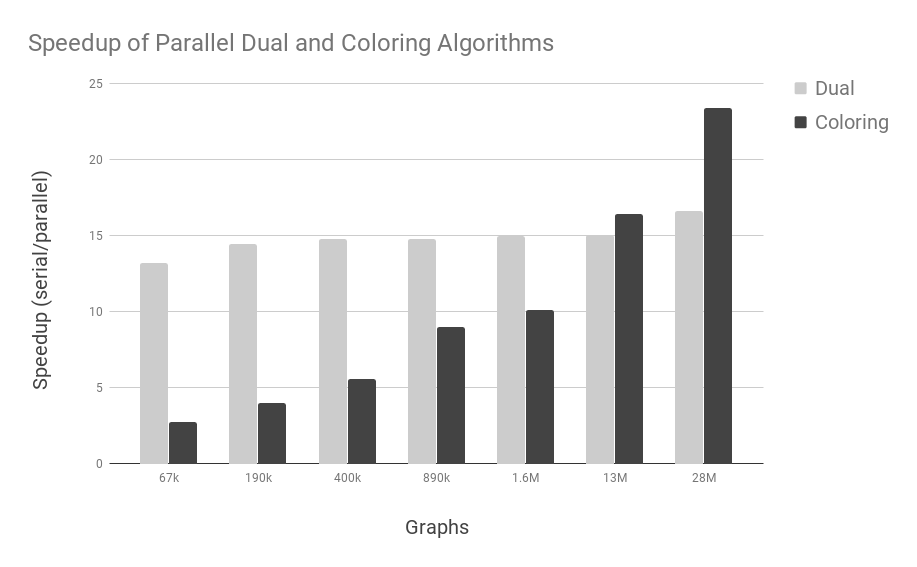
\includegraphics[width=3in]{images/Parallel_Speedup.png}
	\caption{The ratio of serial time compared to parallel for eve construction and coloring }
	\label{fig:edgecounts}
\end{figure}
The timing speedup results shown in \textbf{Fig. 2} demonstrate that parallelism speeds up both coloring and graph construction. However the speedup to graph construction is nearly constant while the speedup to graph coloring continues to increase with the problem size.

\begin{itemize}
  \item Figure out a better title for this section
  \item flow control strong scaling case with 1.3B tets: \\
64Ki \url{https://zenodo.org/record/833519#.WztuxXWYV1M} \\
128Ki \url{https://zenodo.org/record/834946#.Wztu-HWYV1M} \\
256Ki \url{https://zenodo.org/record/835483#.WztvCXWYV1M} \\
512Ki \url{https://zenodo.org/record/835742#.WztvG3WYV1M}
  \item the number of elements per-process may be too small for nodes with large GPUs to run efficiently (data transfer may become more costly than running the selection on the CPU!) - especially as we approach 512Ki parts
  \item we will have to run the condense tool to create an 2Ki (640k elms/part),
    4Ki (320k), 8Ki (160k), 16Ki (80k), and 32Ki (40k) meshes -
    fun3d uses between 75M and 2.3M elements per GPU on summitdev (from siampp18
    presentation)
  \item run on ORNL titan or summit (if accessible)
  \item compare runtimes versus results from SC17 paper~\cite{engparSC17}
  \item use mesh vertex = graph vertex and mesh edge = graph edge for tests -
    will need to run MPI only engpar to establish the baseline performance
  \item plot the time spent in MPI only selection vs kokkos coloring selection
    vs part size - the comparison must start and end at equivalent points in the
    code - start before selection and end just before migration (or whatever the
    next stage) begins
  \item plot the breakdown of time spent in coloring selection vs part size -
    data transfer, color computation, selection (possibly broken into cavity
    selection and filtering for distance), tranferring the selection list
    back to the host
  \item I expect there will be some reduction in partition quality using the
    coloring based selection since we won't have as fine-grained control over
    the process as the MPI only procedure.  As long as the quality reduction is
    controlled and performance is better we should be OK.
\end{itemize}

\section{Closing Remarks} \label{sec:closing}
\begin{itemize}
  \item summarize results
  \item discuss hypergraph coloring and relation to distance-2 coloring for non-simplices (quads, hexs, prisms, pyramids, etc.)
\end{itemize}

\begin{acknowledgement}
This research was supported by the U.S. Department of Energy, Office of Science,
Office of Advanced Scientific Computing Research, under award DE-SC00066117
(FASTMath SciDAC Institute) and by the National Science Foundation under Grant
No. ACI 1533581, (SI2-SSE: Fast Dynamic Load Balancing Tools for Extreme Scale
Systems).

We gratefully acknowledge the use of the resources of the ABC and the XYZ.

Any opinions, findings, and conclusions or recommendations expressed in this
material are those of the author(s) and do not necessarily reflect the views
of the National Science Foundation.
\end{acknowledgement}

\bibliographystyle{acm}
\bibliography{scorec-refs/scorec-refs}
\end{document}
